\documentclass[12pt, xcolor=table]{beamer}
\usepackage{graphicx}
\usepackage[ngerman]{babel}
\usepackage[utf8]{inputenc}
%\usepackage[T1]{fontenc}
\usepackage{amsmath}
\usepackage{amssymb}
\usepackage{listings}
\usepackage{hyperref}
\usepackage{fancyvrb}
\usepackage{color}
\usepackage{verbatim}
\usepackage{alltt}

\usepackage[percent]{overpic}
\usepackage[footnotesize, bf]{caption}
\usepackage[all]{xy}
%Copyright 2008 by Adrian Böhmichen
%
% This file is free software: you can redistribute it and/or modify
% it under the terms of the GNU General Public License as published by
% the Free Software Foundation, either version 3 of the License, or
% (at your option) any later version.
%
% This file is distributed in the hope that it will be useful,
% but WITHOUT ANY WARRANTY; without even the implied warranty of
% MERCHANTABILITY or FITNESS FOR A PARTICULAR PURPOSE.  See the
% GNU General Public License for more details.
%
% You should have received a copy of the GNU General Public License
% along with this file.  If not, see <http://www.gnu.org/licenses/>.

%%%%%%%%%%%%%%%%%%%%%%%%%%%%%%%%%%%%%%%%%%%%%%%%%%%%%%%%%%%%%%%%%
%     Ubuntuusers Vorlage für ein LaTeX-Beamer Theme            %
%                                                               %
% Für das Korrekte funktionieren benötigt man einen header.png  %
% und ein logo.png Datei!                                       %
% Zusätzlich muss man folgende Pakete benutzten:                %
%   \usepackage{graphicx}                                       %
%   \usepackage[percent]{overpic}                               %
%                                                               %
% Danach muss nur noch am Anfang die Datei                      %
% mit \input{} eingebunden werden.                              %
%                                                               %
%%%%%%%%%%%%%%%%%%%%%%%%%%%%%%%%%%%%%%%%%%%%%%%%%%%%%%%%%%%%%%%%%

%weitere Farbe spezifizieren:
%Farben von dem Humantheme
%\definecolor{Orange}{RGB}{240,165,19}
\definecolor{Orange}{RGB}{5,215,242}
%\definecolor{Human-Base}{RGB}{129,102,71}
\definecolor{Human-Base}{RGB}{5,25,242}
%Farben aus dem Inyokatheme
%\definecolor{uuheader1}{RGB}{164,143,101}
\definecolor{uuheader1}{RGB}{5,25,242}
%\definecolor{uuheader2}{RGB}{129,106,59}
\definecolor{uuheader2}{RGB}{5,25,242}


%Theme festlegen für alle Templates die nicht selbstständig definiert werden:
\usepackage{beamerthemedefault}


%Definieren des Innertheme, zuständig für die Symbole bei Listen
\setbeamertemplate{sections/subsections in toc}[circle]
\setbeamertemplate{items}[circle]

\setbeamercolor{item}{fg=Human-Base}

%entfernen der Navigationsleiste
\beamertemplatenavigationsymbolsempty

%Logo definieren, man kann die Lage nicht verändern
%\logo{\includegraphics[scale=0.1]{logo.png}}


%Kopf- und Fußzeile definieren
%\setbeamertemplate{headline}
%{%
%\begin{overpic}[width=\paperwidth
% nächste Zeile dient zum anzeigen eines Rasters, für das paltzieren des ToC hilfreich
%,grid,tics=10
%]
%{header.png}%
%  \put(0,11){\insertsectionnavigationhorizontal{\paperwidth}{~}{~}}%
%  \end{overpic}
%}

\setbeamertemplate{footline}[text line]
{%
\begin{minipage}[b]{116mm}
\insertauthor \hfill%
%neue Navigationsleiste
 \insertframenumber ~/ \inserttotalframenumber\\[1ex]
\end{minipage}
}

% Farben festlegen ausserhalb des innertheme

%Allgemeine Angaben und Verbesserung vom default Theme
\setbeamercolor{structure}{fg=uuheader1}
\setbeamercolor{section in toc}{fg=Human-Base}
\setbeamercolor{subsection in toc}{parent=section in toc}
\setbeamercolor{framesubtitle}{fg=uuheader2}


%Farbe und Form der Blöcke definieren
\setbeamertemplate{blocks}[rounded]
%\setbeamercolor{block title}{fg=uuheader1,bg=Orange}
%\setbeamercolor{block title alerted}{use=alerted text,fg=black,bg=alerted text.fg!75!bg}
%\setbeamercolor{block title example}{use=example text,fg=black,bg=example text.fg!75!bg}

%\setbeamercolor{block body}{parent=normal text,use=block title,bg=block title.bg!25!bg}
%\setbeamercolor{block body alerted}{parent=normal text,use=block title alerted,bg=block title alerted.bg!25!bg}
%\setbeamercolor{block body example}{parent=normal text,use=block title example,bg=block title example.bg!25!bg}

%Für den Titleframe
\setbeamertemplate{title page}[default][rounded=true]
\setbeamercolor{title}{fg=uuheader2}
%,bg=Orange}


\makeatletter
\def\PY@reset{\let\PY@it=\relax \let\PY@bf=\relax%
    \let\PY@ul=\relax \let\PY@tc=\relax%
    \let\PY@bc=\relax \let\PY@ff=\relax}
\def\PY@tok#1{\csname PY@tok@#1\endcsname}
\def\PY@toks#1+{\ifx\relax#1\empty\else%
    \PY@tok{#1}\expandafter\PY@toks\fi}
\def\PY@do#1{\PY@bc{\PY@tc{\PY@ul{%
    \PY@it{\PY@bf{\PY@ff{#1}}}}}}}
\def\PY#1#2{\PY@reset\PY@toks#1+\relax+\PY@do{#2}}

\def\PY@tok@gd{\def\PY@tc##1{\textcolor[rgb]{0.63,0.00,0.00}{##1}}}
\def\PY@tok@gu{\let\PY@bf=\textbf\def\PY@tc##1{\textcolor[rgb]{0.50,0.00,0.50}{##1}}}
\def\PY@tok@gt{\def\PY@tc##1{\textcolor[rgb]{0.00,0.25,0.82}{##1}}}
\def\PY@tok@gs{\let\PY@bf=\textbf}
\def\PY@tok@gr{\def\PY@tc##1{\textcolor[rgb]{1.00,0.00,0.00}{##1}}}
\def\PY@tok@cm{\let\PY@it=\textit\def\PY@tc##1{\textcolor[rgb]{0.25,0.50,0.50}{##1}}}
\def\PY@tok@vg{\def\PY@tc##1{\textcolor[rgb]{0.10,0.09,0.49}{##1}}}
\def\PY@tok@m{\def\PY@tc##1{\textcolor[rgb]{0.40,0.40,0.40}{##1}}}
\def\PY@tok@mh{\def\PY@tc##1{\textcolor[rgb]{0.40,0.40,0.40}{##1}}}
\def\PY@tok@go{\def\PY@tc##1{\textcolor[rgb]{0.50,0.50,0.50}{##1}}}
\def\PY@tok@ge{\let\PY@it=\textit}
\def\PY@tok@vc{\def\PY@tc##1{\textcolor[rgb]{0.10,0.09,0.49}{##1}}}
\def\PY@tok@il{\def\PY@tc##1{\textcolor[rgb]{0.40,0.40,0.40}{##1}}}
\def\PY@tok@cs{\let\PY@it=\textit\def\PY@tc##1{\textcolor[rgb]{0.25,0.50,0.50}{##1}}}
\def\PY@tok@cp{\def\PY@tc##1{\textcolor[rgb]{0.74,0.48,0.00}{##1}}}
\def\PY@tok@gi{\def\PY@tc##1{\textcolor[rgb]{0.00,0.63,0.00}{##1}}}
\def\PY@tok@gh{\let\PY@bf=\textbf\def\PY@tc##1{\textcolor[rgb]{0.00,0.00,0.50}{##1}}}
\def\PY@tok@ni{\let\PY@bf=\textbf\def\PY@tc##1{\textcolor[rgb]{0.60,0.60,0.60}{##1}}}
\def\PY@tok@nl{\def\PY@tc##1{\textcolor[rgb]{0.63,0.63,0.00}{##1}}}
\def\PY@tok@nn{\let\PY@bf=\textbf\def\PY@tc##1{\textcolor[rgb]{0.00,0.00,1.00}{##1}}}
\def\PY@tok@no{\def\PY@tc##1{\textcolor[rgb]{0.53,0.00,0.00}{##1}}}
\def\PY@tok@na{\def\PY@tc##1{\textcolor[rgb]{0.49,0.56,0.16}{##1}}}
\def\PY@tok@nb{\def\PY@tc##1{\textcolor[rgb]{0.00,0.50,0.00}{##1}}}
\def\PY@tok@nc{\let\PY@bf=\textbf\def\PY@tc##1{\textcolor[rgb]{0.00,0.00,1.00}{##1}}}
\def\PY@tok@nd{\def\PY@tc##1{\textcolor[rgb]{0.67,0.13,1.00}{##1}}}
\def\PY@tok@ne{\let\PY@bf=\textbf\def\PY@tc##1{\textcolor[rgb]{0.82,0.25,0.23}{##1}}}
\def\PY@tok@nf{\def\PY@tc##1{\textcolor[rgb]{0.00,0.00,1.00}{##1}}}
\def\PY@tok@si{\let\PY@bf=\textbf\def\PY@tc##1{\textcolor[rgb]{0.73,0.40,0.53}{##1}}}
\def\PY@tok@s2{\def\PY@tc##1{\textcolor[rgb]{0.73,0.13,0.13}{##1}}}
\def\PY@tok@vi{\def\PY@tc##1{\textcolor[rgb]{0.10,0.09,0.49}{##1}}}
\def\PY@tok@nt{\let\PY@bf=\textbf\def\PY@tc##1{\textcolor[rgb]{0.00,0.50,0.00}{##1}}}
\def\PY@tok@nv{\def\PY@tc##1{\textcolor[rgb]{0.10,0.09,0.49}{##1}}}
\def\PY@tok@s1{\def\PY@tc##1{\textcolor[rgb]{0.73,0.13,0.13}{##1}}}
\def\PY@tok@sh{\def\PY@tc##1{\textcolor[rgb]{0.73,0.13,0.13}{##1}}}
\def\PY@tok@sc{\def\PY@tc##1{\textcolor[rgb]{0.73,0.13,0.13}{##1}}}
\def\PY@tok@sx{\def\PY@tc##1{\textcolor[rgb]{0.00,0.50,0.00}{##1}}}
\def\PY@tok@bp{\def\PY@tc##1{\textcolor[rgb]{0.00,0.50,0.00}{##1}}}
\def\PY@tok@c1{\let\PY@it=\textit\def\PY@tc##1{\textcolor[rgb]{0.25,0.50,0.50}{##1}}}
\def\PY@tok@kc{\let\PY@bf=\textbf\def\PY@tc##1{\textcolor[rgb]{0.00,0.50,0.00}{##1}}}
\def\PY@tok@c{\let\PY@it=\textit\def\PY@tc##1{\textcolor[rgb]{0.25,0.50,0.50}{##1}}}
\def\PY@tok@mf{\def\PY@tc##1{\textcolor[rgb]{0.40,0.40,0.40}{##1}}}
\def\PY@tok@err{\def\PY@bc##1{\fcolorbox[rgb]{1.00,0.00,0.00}{1,1,1}{##1}}}
\def\PY@tok@kd{\let\PY@bf=\textbf\def\PY@tc##1{\textcolor[rgb]{0.00,0.50,0.00}{##1}}}
\def\PY@tok@ss{\def\PY@tc##1{\textcolor[rgb]{0.10,0.09,0.49}{##1}}}
\def\PY@tok@sr{\def\PY@tc##1{\textcolor[rgb]{0.73,0.40,0.53}{##1}}}
\def\PY@tok@mo{\def\PY@tc##1{\textcolor[rgb]{0.40,0.40,0.40}{##1}}}
\def\PY@tok@kn{\let\PY@bf=\textbf\def\PY@tc##1{\textcolor[rgb]{0.00,0.50,0.00}{##1}}}
\def\PY@tok@mi{\def\PY@tc##1{\textcolor[rgb]{0.40,0.40,0.40}{##1}}}
\def\PY@tok@gp{\let\PY@bf=\textbf\def\PY@tc##1{\textcolor[rgb]{0.00,0.00,0.50}{##1}}}
\def\PY@tok@o{\def\PY@tc##1{\textcolor[rgb]{0.40,0.40,0.40}{##1}}}
\def\PY@tok@kr{\let\PY@bf=\textbf\def\PY@tc##1{\textcolor[rgb]{0.00,0.50,0.00}{##1}}}
\def\PY@tok@s{\def\PY@tc##1{\textcolor[rgb]{0.73,0.13,0.13}{##1}}}
\def\PY@tok@kp{\def\PY@tc##1{\textcolor[rgb]{0.00,0.50,0.00}{##1}}}
\def\PY@tok@w{\def\PY@tc##1{\textcolor[rgb]{0.73,0.73,0.73}{##1}}}
\def\PY@tok@kt{\def\PY@tc##1{\textcolor[rgb]{0.69,0.00,0.25}{##1}}}
\def\PY@tok@ow{\let\PY@bf=\textbf\def\PY@tc##1{\textcolor[rgb]{0.67,0.13,1.00}{##1}}}
\def\PY@tok@sb{\def\PY@tc##1{\textcolor[rgb]{0.73,0.13,0.13}{##1}}}
\def\PY@tok@k{\let\PY@bf=\textbf\def\PY@tc##1{\textcolor[rgb]{0.00,0.50,0.00}{##1}}}
\def\PY@tok@se{\let\PY@bf=\textbf\def\PY@tc##1{\textcolor[rgb]{0.73,0.40,0.13}{##1}}}
\def\PY@tok@sd{\let\PY@it=\textit\def\PY@tc##1{\textcolor[rgb]{0.73,0.13,0.13}{##1}}}

\def\PYZbs{\char`\\}
\def\PYZus{\char`\_}
\def\PYZob{\char`\{}
\def\PYZcb{\char`\}}
\def\PYZca{\char`\^}
\def\PYZsh{\char`\#}
\def\PYZpc{\char`\%}
\def\PYZdl{\char`\$}
\def\PYZti{\char`\~}
% for compatibility with earlier versions
\def\PYZat{@}
\def\PYZlb{[}
\def\PYZrb{]}
\makeatother

\renewcommand{\footnotesize}{\tiny}

\begin{document}
\title{Mapping Between Categories: On Functors in Functional Programming}
\author{Lusy}
\date{\today}

\begin{frame}
    \titlepage
    \begin{block}
        \tiny \url{https://github.com/lusy/functorsTalk}
    \end{block}
\end{frame}

\section{Introduction} % (fold)
\begin{frame}
     \frametitle{Introduction}
     % Find a picture to backup the introductory questions
     %* how many people have already seen/done some functional programming?
     %* how many of them are familiar with Haskell?
     %* does anybody know what Functors are?
     \begin{center}
         
\includegraphics[scale=0.4]{figures/pickme.png}
     \end{center}
\end{frame}

%\begin{comment}
%\begin{frame}
%    \frametitle{Why is functional programming awesome?}
%    \begin{itemize}
%        \item immutability %excel picture
%        \item concurrency %dinning philosophers
%        \item elegancy
%        %\item first class functions
%    \end{itemize}
%    % code example
%    % excel example for the immutability
%\end{frame}
%\ende{comment}

%\begin{frame}
%    \frametitle{Why is functional programming awesome?}
%    \begin{block}{Immutability + Concurrency}
%        \begin{center}
%            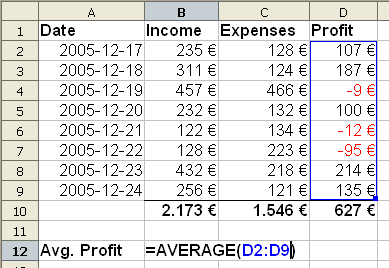
\includegraphics[scale=0.4]{figures/Spreadsheet.png}
%        \end{center}
%    \end{block}
    % code example
    % excel example for the immutability
%\end{frame}

%\begin{frame}
%    \frametitle{Why is functional programming awesome?}
%    \begin{block}{Concurrency}
%        \begin{center}
%            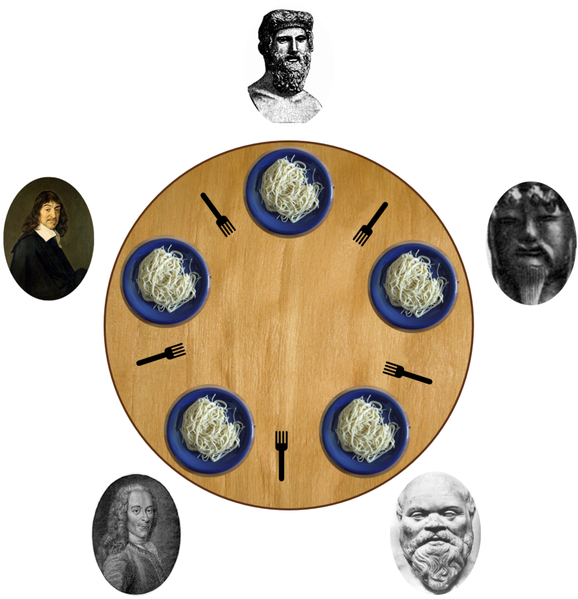
\includegraphics[scale=0.3]{figures/DiningPhilosophers.png}
%        \end{center}
%    \end{block}
    % code example
    % excel example for the immutability
%\end{frame}

%\begin{frame}
%    \frametitle{Why is functional programming awesome?}
%    \begin{block}{Elegancy}
%        \begin{block}{Haskell}
%                \begin{alltt}
%                    \begin{tiny}
%                    qsort :: Ord a => [a] -> [a]
%                    \newline
%                    qsort []     = []
%                    \newline
%                    qsort (x:xs) = qsort (filter (< x) xs) ++ [x] ++ qsort (filter (>= x) xs)
%                \end{tiny}
%                \end{alltt}
%        \end{block}
%        \begin{block}{Javascript}
%                \begin{alltt}
%                    \begin{tiny}
%                    function qsort(a) \{ \\
%                        if (a.length == 0) return []; \\
%
%                        var left = [], right = [], pivot = a[0];\\
%
%                        for (var i = 1; i < a.length; i++) \{ \\
%                            a[i] < pivot ? left.push(a[i]) : right.push(a[i]); \\
%                        \} \\
%
%                        return qsort(left).concat(pivot, qsort(right)); \\
%                    \}
%                    \end{tiny}
%                \end{alltt}
%        \end{block}
%    \end{block}
%\end{frame}

\begin{frame}
    \frametitle{Some Maths}
        \begin{block}{Category Theory}
        \begin{itemize}
            \item mathematical abstraction
            \item categories are sets, vector spaces, or types for computer science..
        \end{itemize}
        \end{block}
        \vspace{30px}
        \hspace*{\fill}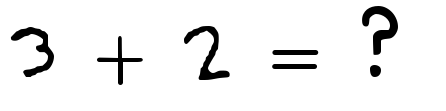
\includegraphics[scale=0.3]{figures/maths.png}
\end{frame}

\begin{frame}
    \frametitle{Category Theory 2}
    \begin{itemize}
        \item there are mappings between them: an object can be ``transferred'' from one category to another
        \item  mappings are structure preservent
    \end{itemize}
    \begin{center}
        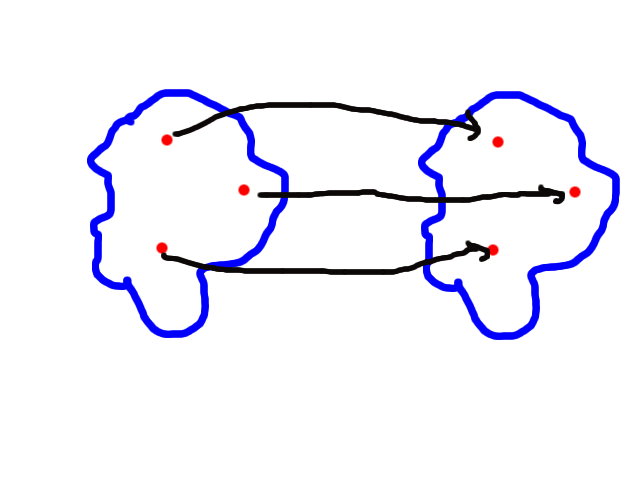
\includegraphics[scale=0.3]{figures/structurePreserv.png}
    \end{center}
\end{frame}

\section{Functors Definition}
\begin{frame}
    \frametitle{So what are functors?}
    Structure preservent mappings between categories!
%    \newline
%    \newline
%    ``A functor associates to every object of one category an object of another category, and to every morphism in the first category a morphism in the second.''
\end{frame}

\begin{frame}
    \frametitle{The Haskell definition}
    ``Types that can act like a box can be functors. You can think of a list as a box that can be empty or have something inside it, including another box!''
    \vspace{30px}
    \begin{columns}
        \column{0.5\textwidth}
            \begin{center}
            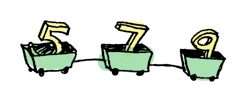
\includegraphics[scale=0.4]{figures/list.png}
            \end{center}
        \column{0.5\textwidth}
            \begin{center}
            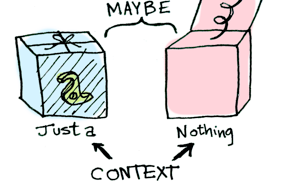
\includegraphics[scale=0.4]{figures/maybe.png}
            \end{center}
    \end{columns}
\end{frame}

\section{Haskell Functors}
\begin{frame}
    \frametitle{The Haskell Definition 2}
    Functor is a type class. Very much like Eq, Ord, Show, ...
    It requires a type constructor that takes \textbf{one} parameter

    \begin{alltt}
        > class  Functor    f   where \\
        >       fmap         ::   (a $\to$ b) $\to$ f a $\to$ f b
%               \newline
%               \newline
%        fmap id           =  id \\
%        fmap (g . f)      =  fmap g . fmap f
    \end{alltt}
    \begin{center}
        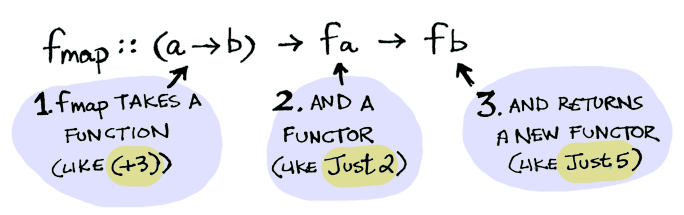
\includegraphics[scale=0.4]{figures/fmapdef.png}
    \end{center}
\end{frame}

\begin{frame}
    \frametitle{An Example - Lists}

    \begin{alltt}
        > map :: (a $\to$ b) $\to$ [a] $\to$ [b] \\
        > instance Functor [] where \\
        >   fmap = map
    \end{alltt}

    \begin{center}
        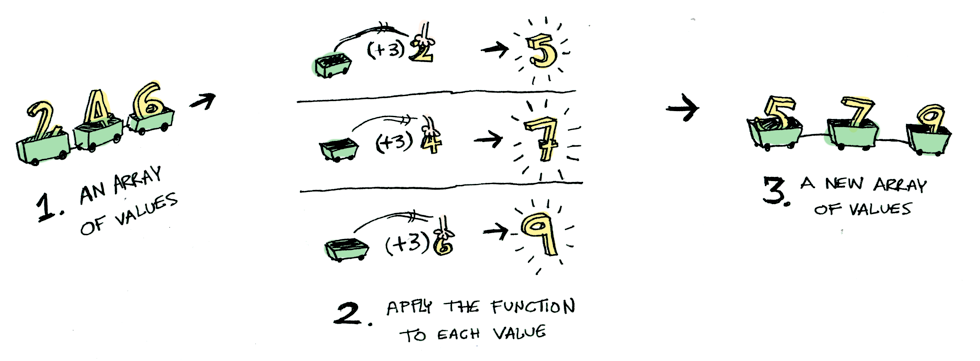
\includegraphics[scale=0.3]{figures/fmapList.png}
    \end{center}
\end{frame}

\begin{frame}{Demo!}
        \begin{alltt}
            > fmap (2 +) [1,2,3]
        \end{alltt}
\end{frame}

\begin{comment}
Further examples

Maybe
-----
> data Maybe x = Just x | Nothing

> instance Functor Maybe where
>   fmap f (Just x) = Just (f x)
>   fmap f Nothing = Nothing


> fmap (++ "ho") (Just "hey")

Trees
-----
> data Tree x = Empty | Node x (Tree x) (Tree x)

> instance Functor Tree where
>   fmap f Empty = Empty
>   fmap f (Node x left right) = Node (f x) (fmap f left) (fmap f right)
\end{comment}

\begin{frame}
    \frametitle{You already know this!}
    % ruby / javascript examples
    \begin{block}{Ruby}
        \begin{alltt}
            [1, 2, 3].map \{ |n| n * n \}
            \newline
            \newline
            => [1, 4, 9]
        \end{alltt}
    \end{block}
\end{frame}

\begin{frame}
    \frametitle{You already know this!}
    % ruby / javascript examples
    \begin{block}{Javascript}
        \begin{alltt}
            \_.map([1, 2, 3], function(num)\{return num*3;\});
            \newline
            \newline
            => [3, 6, 9]
        \end{alltt}
    \end{block}
\end{frame}

\begin{frame}
    \frametitle{From a functor to another functor}
    \begin{block}{Tree vs Array}
    \begin{columns}
        \column{0.5\textwidth}
            \begin{center}
            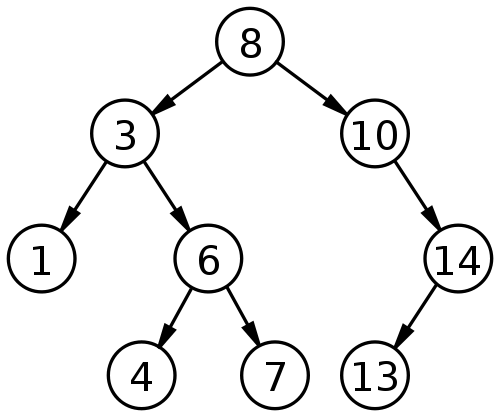
\includegraphics[scale=0.3]{figures/tree.png}
            \end{center}
        \column{0.5\textwidth}
            \begin{center}
                [1, 3, 4, 6, 7, 8, 10, 13, 14]
            \end{center}
    \end{columns}
\end{block}
\end{frame}

\begin{frame}
    \frametitle{The Natural Transformation}
    % Mapping between functors
            \begin{equation*}
                   \xymatrix@C+2em@R+2em{
                      F(A) \ar[r]^{fmap\_f} \ar[d]_{\alpha_A} & F(B) \ar[d]^{\alpha_B} \\
                      G(A) \ar[r]_{fmap\_g} & G(B)
                     }
            \end{equation*}

%            $\alpha :: F a \ar G a$
%            Parametricity:
%            $\alpha . fmap\_f = fmap\_f . \alpha$

\end{frame}


\section{The end..} % (fold)
\begin{frame}
    \frametitle{The End...}
    \begin{block}{Thanks!}
        Questions?
    \end{block}
\end{frame}

\section{Picture Sources}
\begin{frame}
    \frametitle{Some Sources}
    \begin{itemize}
        \item \tiny{http://learnyouahaskell.com/}
        \item \tiny{http://adit.io/posts/2013-04-17-functors,\_applicatives,\_and\_monads\_in\_pictures.html}
        %\item \tiny{https://en.wikipedia.org/wiki/File:Dining\_philosophers.png}
        %\item \tiny{https://commons.wikimedia.org/wiki/File:Spreadsheet.png}
        %\item \tiny{https://en.wikibooks.org/wiki/Algorithm\_Implementation/Sorting/Quicksort}
        \item \tiny{https://en.wikipedia.org/wiki/File:Binary\_search\_tree.svg}
        \item \tiny{https://en.wikipedia.org/wiki/Category\_theory}
    \end{itemize}
\end{frame}

\end{document}
